\documentclass{standalone}
\usepackage{tikz}
\usetikzlibrary{patterns}
\usetikzlibrary{positioning}
\usetikzlibrary{patterns, positioning}
\usetikzlibrary{shapes.misc}
\usepackage[outline]{contour}
\contourlength{1.5pt} 
\usetikzlibrary{calc}
        \usepackage{relsize}
        \tikzset{fontscale/.style = {font=\relsize{#1}}}

\begin{document}
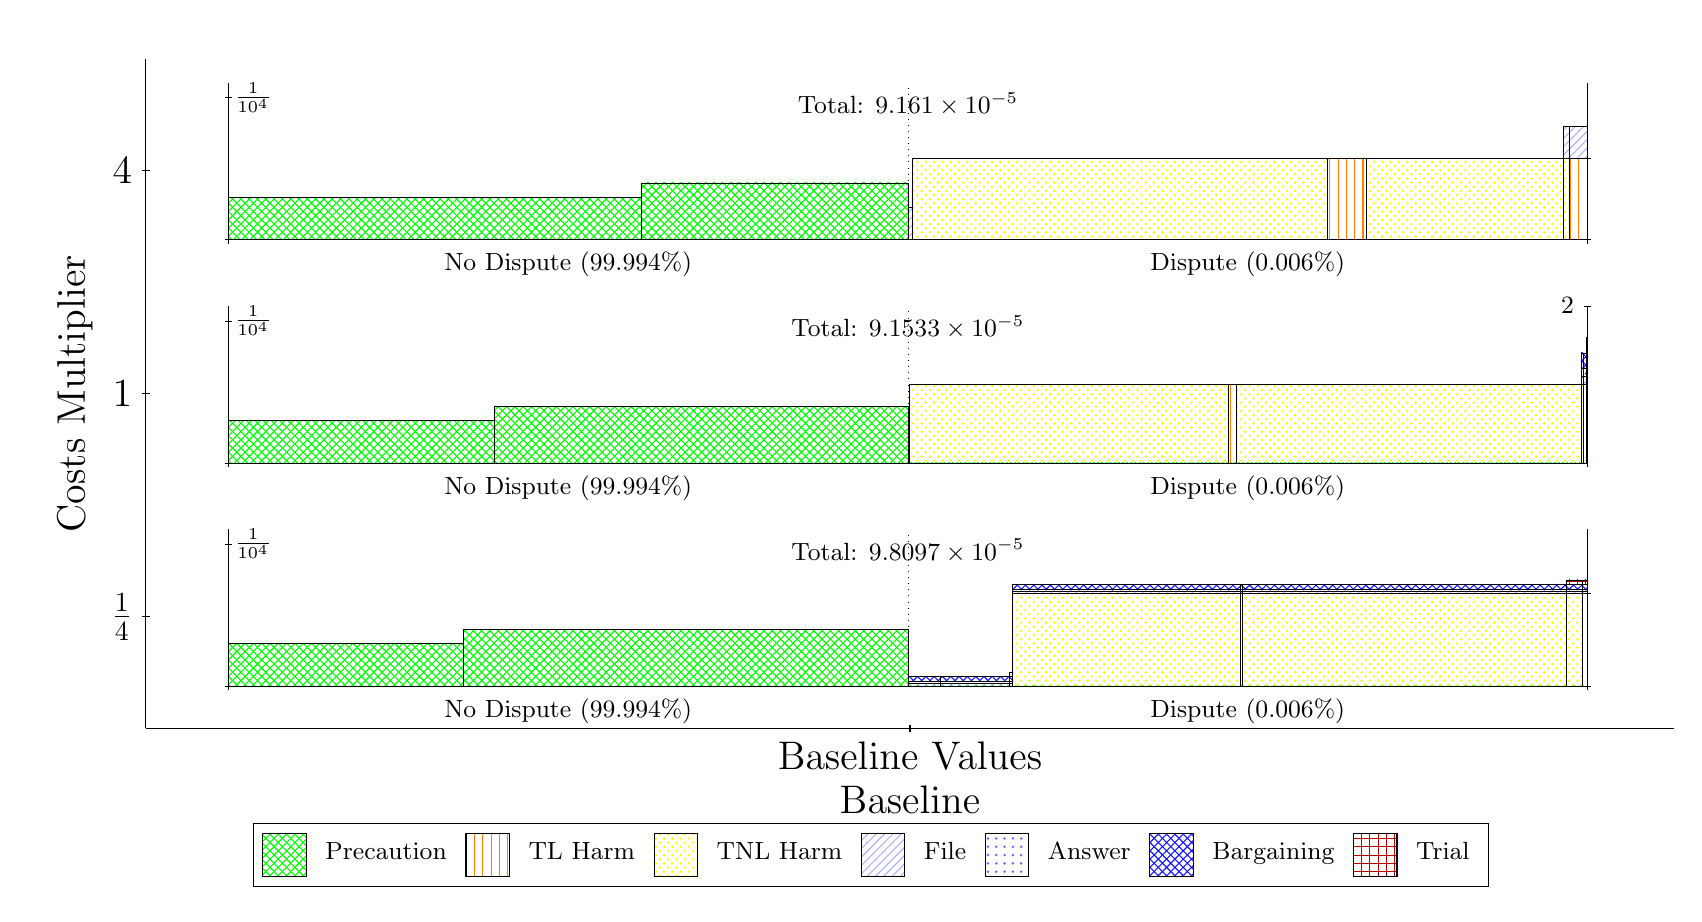
\begin{tikzpicture}
\clip(-0.5,-1.1) rectangle +(20.91,11);
\draw[black] (1,1) -- (1,9.5);
\node[rotate=90, fontscale=2, anchor=center] at (0.1, 5.25) {Costs Multiplier};
\draw[black] (0.95,2.4167) -- (1.05,2.4167);
\node[fontscale=2, anchor=east] at (0.95, 2.4167) {$\frac{1}{4}$};
\draw[black] (0.95,5.25) -- (1.05,5.25);
\node[fontscale=2, anchor=east] at (0.95, 5.25) {1};
\draw[black] (0.95,8.0833) -- (1.05,8.0833);
\node[fontscale=2, anchor=east] at (0.95, 8.0833) {4};

\draw[black] (1,1) -- (20.41,1);
\node[fontscale=2, anchor=center] at (10.705, 0.1) {Baseline};
\draw[black] (10.705,0.95) -- (10.705,1.05);
\node[fontscale=2, anchor=north] at (10.705, 0.95) {Baseline Values};


\draw[pattern=crosshatch, pattern color=green,draw=black,very thin] (2.05,1.54) rectangle (5.0364,2.0809);
\draw[pattern=crosshatch, pattern color=green,draw=black,very thin] (5.0364,1.54) rectangle (10.68,2.2612);
\draw[pattern=crosshatch, pattern color=green,draw=black,very thin] (10.68,1.54) rectangle (11.094,1.54);
\draw[pattern=north east lines, pattern color=blue!30,draw=black,very thin] (10.68,1.54) rectangle (11.094,1.5693);
\draw[pattern=dots,  pattern color=blue!60,draw=black,very thin] (10.68,1.5693) rectangle (11.094,1.5986);
\draw[pattern=crosshatch,      pattern color=blue!90,draw=black,very thin] (10.68,1.5986) rectangle (11.094,1.6571);
\draw[pattern=crosshatch, pattern color=green,draw=black,very thin] (11.094,1.54) rectangle (11.963,1.54);
\draw[pattern=north east lines, pattern color=blue!30,draw=black,very thin] (11.094,1.54) rectangle (11.963,1.5693);
\draw[pattern=dots,  pattern color=blue!60,draw=black,very thin] (11.094,1.5693) rectangle (11.963,1.5986);
\draw[pattern=crosshatch,      pattern color=blue!90,draw=black,very thin] (11.094,1.5986) rectangle (11.963,1.6572);
\draw[pattern=crosshatch, pattern color=green,draw=black,very thin] (11.963,1.54) rectangle (12.009,1.54);
\draw[pattern=north east lines, pattern color=blue!30,draw=black,very thin] (11.963,1.54) rectangle (12.009,1.5693);
\draw[pattern=dots,  pattern color=blue!60,draw=black,very thin] (11.963,1.5693) rectangle (12.009,1.5986);
\draw[pattern=crosshatch,      pattern color=blue!90,draw=black,very thin] (11.963,1.5986) rectangle (12.009,1.6571);
\draw[pattern=grid,            pattern color=red!70!black,draw=black,very thin] (11.963,1.6571) rectangle (12.009,1.7157);
\draw[pattern=crosshatch, pattern color=green,draw=black,very thin] (12.009,1.54) rectangle (14.902,1.54);
\draw[pattern=crosshatch dots, pattern color=yellow,draw=black,very thin] (12.009,1.54) rectangle (14.902,2.7111);
\draw[pattern=north east lines, pattern color=blue!30,draw=black,very thin] (12.009,2.7111) rectangle (14.902,2.7404);
\draw[pattern=dots,  pattern color=blue!60,draw=black,very thin] (12.009,2.7404) rectangle (14.902,2.7696);
\draw[pattern=crosshatch,      pattern color=blue!90,draw=black,very thin] (12.009,2.7696) rectangle (14.902,2.8282);
\draw[pattern=crosshatch, pattern color=green,draw=black,very thin] (14.902,1.54) rectangle (14.929,1.54);
\draw[pattern=vertical lines, pattern color=orange,draw=black,very thin] (14.902,1.54) rectangle (14.929,2.7111);
\draw[pattern=north east lines, pattern color=blue!30,draw=black,very thin] (14.902,2.7111) rectangle (14.929,2.7404);
\draw[pattern=dots,  pattern color=blue!60,draw=black,very thin] (14.902,2.7404) rectangle (14.929,2.7696);
\draw[pattern=crosshatch,      pattern color=blue!90,draw=black,very thin] (14.902,2.7696) rectangle (14.929,2.8282);
\draw[pattern=crosshatch, pattern color=green,draw=black,very thin] (14.929,1.54) rectangle (19.034,1.54);
\draw[pattern=crosshatch dots, pattern color=yellow,draw=black,very thin] (14.929,1.54) rectangle (19.034,2.7111);
\draw[pattern=north east lines, pattern color=blue!30,draw=black,very thin] (14.929,2.7111) rectangle (19.034,2.7404);
\draw[pattern=dots,  pattern color=blue!60,draw=black,very thin] (14.929,2.7404) rectangle (19.034,2.7697);
\draw[pattern=crosshatch,      pattern color=blue!90,draw=black,very thin] (14.929,2.7697) rectangle (19.034,2.8282);
\draw[pattern=crosshatch, pattern color=green,draw=black,very thin] (19.034,1.54) rectangle (19.241,1.54);
\draw[pattern=crosshatch dots, pattern color=yellow,draw=black,very thin] (19.034,1.54) rectangle (19.241,2.7111);
\draw[pattern=north east lines, pattern color=blue!30,draw=black,very thin] (19.034,2.7111) rectangle (19.241,2.7404);
\draw[pattern=dots,  pattern color=blue!60,draw=black,very thin] (19.034,2.7404) rectangle (19.241,2.7696);
\draw[pattern=crosshatch,      pattern color=blue!90,draw=black,very thin] (19.034,2.7696) rectangle (19.241,2.8282);
\draw[pattern=grid,            pattern color=red!70!black,draw=black,very thin] (19.034,2.8282) rectangle (19.241,2.8868);
\draw[pattern=crosshatch, pattern color=green,draw=black,very thin] (19.241,1.54) rectangle (19.31,1.54);
\draw[pattern=vertical lines, pattern color=orange,draw=black,very thin] (19.241,1.54) rectangle (19.31,2.7111);
\draw[pattern=north east lines, pattern color=blue!30,draw=black,very thin] (19.241,2.7111) rectangle (19.31,2.7404);
\draw[pattern=dots,  pattern color=blue!60,draw=black,very thin] (19.241,2.7404) rectangle (19.31,2.7696);
\draw[pattern=crosshatch,      pattern color=blue!90,draw=black,very thin] (19.241,2.7696) rectangle (19.31,2.8282);
\draw[pattern=grid,            pattern color=red!70!black,draw=black,very thin] (19.241,2.8282) rectangle (19.31,2.8868);
\node[font=\small,text=black,anchor=north] at (10.68, 3.5333) {Total: $9.8097\times 10^{-5}$};
\draw[black,very thin] (2.05,1.54) -- (2.05,3.5333);
\draw[black,very thin] (2,1.54) -- (2.1,1.54);
\node[font=\small,text=black, anchor=west] at (2, 1.54) {};
\draw[black,very thin] (2,3.3431) -- (2.1,3.3431);
\node[font=\small,text=black, anchor=west] at (2, 3.3431) {$\frac{1}{10^{4}}$};

\draw[black,dotted,very thin] (10.68,1.5998) -- (10.68,3.4735);
\draw[black,very thin] (19.31,1.54) -- (19.31,3.5333);
\draw[black,very thin] (19.26,1.54) -- (19.36,1.54);
\node[font=\small,text=black, anchor=east] at (19.26, 1.54) {\contour{white}{}};
\draw[black,very thin] (19.26,2.7111) -- (19.36,2.7111);
\node[font=\small,text=black, anchor=east] at (19.26, 2.7111) {\contour{white}{}};

\draw[black,very thin] (2.05,1.54) -- (19.31,1.54);
\draw[black,very thin] (2.05,1.49) -- (2.05,1.59);
\node[font=\small,text=black, anchor=north] at (2.05, 1.49) {};
\draw[black,very thin] (19.31,1.49) -- (19.31,1.59);
\node[font=\small,text=black, anchor=north] at (19.31, 1.49) {};

\node[font=\small,text=black,anchor=south] at (6.365, 0.94) {No\ Dispute\ (99.994\%)};
\node[font=\small,text=black,anchor=south] at (14.995, 0.94) {Dispute\ (0.006\%)};

\draw[pattern=crosshatch, pattern color=green,draw=black,very thin] (2.05,4.3733) rectangle (5.4319,4.9143);
\draw[pattern=crosshatch, pattern color=green,draw=black,very thin] (5.4319,4.3733) rectangle (10.68,5.0946);
\draw[pattern=crosshatch, pattern color=green,draw=black,very thin] (10.68,4.3733) rectangle (10.692,4.3734);
\draw[pattern=north east lines, pattern color=blue!30,draw=black,very thin] (10.68,4.3734) rectangle (10.692,4.473);
\draw[pattern=dots,  pattern color=blue!60,draw=black,very thin] (10.68,4.473) rectangle (10.692,4.5727);
\draw[pattern=crosshatch,      pattern color=blue!90,draw=black,very thin] (10.68,4.5727) rectangle (10.692,4.772);
\draw[pattern=crosshatch, pattern color=green,draw=black,very thin] (10.692,4.3733) rectangle (14.748,4.3734);
\draw[pattern=crosshatch dots, pattern color=yellow,draw=black,very thin] (10.692,4.3734) rectangle (14.748,5.37);
\draw[pattern=crosshatch, pattern color=green,draw=black,very thin] (14.748,4.3733) rectangle (14.846,4.3734);
\draw[pattern=vertical lines, pattern color=orange,draw=black,very thin] (14.748,4.3734) rectangle (14.846,5.37);
\draw[pattern=crosshatch, pattern color=green,draw=black,very thin] (14.846,4.3733) rectangle (19.227,4.3734);
\draw[pattern=crosshatch dots, pattern color=yellow,draw=black,very thin] (14.846,4.3734) rectangle (19.227,5.37);
\draw[pattern=crosshatch, pattern color=green,draw=black,very thin] (19.227,4.3733) rectangle (19.258,4.3734);
\draw[pattern=crosshatch dots, pattern color=yellow,draw=black,very thin] (19.227,4.3734) rectangle (19.258,5.37);
\draw[pattern=north east lines, pattern color=blue!30,draw=black,very thin] (19.227,5.37) rectangle (19.258,5.4697);
\draw[pattern=dots,  pattern color=blue!60,draw=black,very thin] (19.227,5.4697) rectangle (19.258,5.5693);
\draw[pattern=crosshatch,      pattern color=blue!90,draw=black,very thin] (19.227,5.5693) rectangle (19.258,5.7687);
\draw[pattern=crosshatch, pattern color=green,draw=black,very thin] (19.258,4.3733) rectangle (19.296,4.3734);
\draw[pattern=vertical lines, pattern color=orange,draw=black,very thin] (19.258,4.3734) rectangle (19.296,5.37);
\draw[pattern=north east lines, pattern color=blue!30,draw=black,very thin] (19.258,5.37) rectangle (19.296,5.4697);
\draw[pattern=dots,  pattern color=blue!60,draw=black,very thin] (19.258,5.4697) rectangle (19.296,5.5693);
\draw[pattern=crosshatch,      pattern color=blue!90,draw=black,very thin] (19.258,5.5693) rectangle (19.296,5.7687);
\draw[pattern=crosshatch, pattern color=green,draw=black,very thin] (19.296,4.3733) rectangle (19.307,4.3734);
\draw[pattern=crosshatch dots, pattern color=yellow,draw=black,very thin] (19.296,4.3734) rectangle (19.307,5.37);
\draw[pattern=north east lines, pattern color=blue!30,draw=black,very thin] (19.296,5.37) rectangle (19.307,5.4697);
\draw[pattern=dots,  pattern color=blue!60,draw=black,very thin] (19.296,5.4697) rectangle (19.307,5.5693);
\draw[pattern=crosshatch,      pattern color=blue!90,draw=black,very thin] (19.296,5.5693) rectangle (19.307,5.7687);
\draw[pattern=grid,            pattern color=red!70!black,draw=black,very thin] (19.296,5.7687) rectangle (19.307,5.968);
\draw[pattern=crosshatch, pattern color=green,draw=black,very thin] (19.307,4.3733) rectangle (19.31,4.3734);
\draw[pattern=vertical lines, pattern color=orange,draw=black,very thin] (19.307,4.3734) rectangle (19.31,5.37);
\draw[pattern=north east lines, pattern color=blue!30,draw=black,very thin] (19.307,5.37) rectangle (19.31,5.4697);
\draw[pattern=dots,  pattern color=blue!60,draw=black,very thin] (19.307,5.4697) rectangle (19.31,5.5693);
\draw[pattern=crosshatch,      pattern color=blue!90,draw=black,very thin] (19.307,5.5693) rectangle (19.31,5.7687);
\draw[pattern=grid,            pattern color=red!70!black,draw=black,very thin] (19.307,5.7687) rectangle (19.31,5.968);
\node[font=\small,text=black,anchor=north] at (10.68, 6.3667) {Total: $9.1533\times 10^{-5}$};
\draw[black,very thin] (2.05,4.3733) -- (2.05,6.3667);
\draw[black,very thin] (2,4.3733) -- (2.1,4.3733);
\node[font=\small,text=black, anchor=west] at (2, 4.3733) {};
\draw[black,very thin] (2,6.1765) -- (2.1,6.1765);
\node[font=\small,text=black, anchor=west] at (2, 6.1765) {$\frac{1}{10^{4}}$};

\draw[black,dotted,very thin] (10.68,4.4331) -- (10.68,6.3069);
\draw[black,very thin] (19.31,4.3733) -- (19.31,6.3667);
\draw[black,very thin] (19.26,6.3666) -- (19.36,6.3666);
\node[font=\small,text=black, anchor=east] at (19.26, 6.3666) {\contour{white}{2}};

\draw[black,very thin] (2.05,4.3733) -- (19.31,4.3733);
\draw[black,very thin] (2.05,4.3233) -- (2.05,4.4233);
\node[font=\small,text=black, anchor=north] at (2.05, 4.3233) {};
\draw[black,very thin] (19.31,4.3233) -- (19.31,4.4233);
\node[font=\small,text=black, anchor=north] at (19.31, 4.3233) {};

\node[font=\small,text=black,anchor=south] at (6.365, 3.7733) {No\ Dispute\ (99.994\%)};
\node[font=\small,text=black,anchor=south] at (14.995, 3.7733) {Dispute\ (0.006\%)};

\draw[pattern=crosshatch, pattern color=green,draw=black,very thin] (2.05,7.2067) rectangle (7.298,7.7476);
\draw[pattern=crosshatch, pattern color=green,draw=black,very thin] (7.298,7.2067) rectangle (10.68,7.9279);
\draw[pattern=crosshatch, pattern color=green,draw=black,very thin] (10.68,7.2067) rectangle (10.737,7.2067);
\draw[pattern=north east lines, pattern color=blue!30,draw=black,very thin] (10.68,7.2067) rectangle (10.737,7.6187);
\draw[pattern=crosshatch, pattern color=green,draw=black,very thin] (10.737,7.2067) rectangle (16.01,7.2067);
\draw[pattern=crosshatch dots, pattern color=yellow,draw=black,very thin] (10.737,7.2067) rectangle (16.01,8.2366);
\draw[pattern=crosshatch, pattern color=green,draw=black,very thin] (16.01,7.2067) rectangle (16.503,7.2067);
\draw[pattern=vertical lines, pattern color=orange,draw=black,very thin] (16.01,7.2067) rectangle (16.503,8.2366);
\draw[pattern=crosshatch, pattern color=green,draw=black,very thin] (16.503,7.2067) rectangle (19.008,7.2067);
\draw[pattern=crosshatch dots, pattern color=yellow,draw=black,very thin] (16.503,7.2067) rectangle (19.008,8.2366);
\draw[pattern=crosshatch, pattern color=green,draw=black,very thin] (19.008,7.2067) rectangle (19.083,7.2067);
\draw[pattern=crosshatch dots, pattern color=yellow,draw=black,very thin] (19.008,7.2067) rectangle (19.083,8.2366);
\draw[pattern=north east lines, pattern color=blue!30,draw=black,very thin] (19.008,8.2366) rectangle (19.083,8.6486);
\draw[pattern=crosshatch, pattern color=green,draw=black,very thin] (19.083,7.2067) rectangle (19.31,7.2067);
\draw[pattern=vertical lines, pattern color=orange,draw=black,very thin] (19.083,7.2067) rectangle (19.31,8.2366);
\draw[pattern=north east lines, pattern color=blue!30,draw=black,very thin] (19.083,8.2366) rectangle (19.31,8.6486);
\node[font=\small,text=black,anchor=north] at (10.68, 9.2) {Total: $9.161\times 10^{-5}$};
\draw[black,very thin] (2.05,7.2067) -- (2.05,9.2);
\draw[black,very thin] (2,7.2067) -- (2.1,7.2067);
\node[font=\small,text=black, anchor=west] at (2, 7.2067) {};
\draw[black,very thin] (2,9.0098) -- (2.1,9.0098);
\node[font=\small,text=black, anchor=west] at (2, 9.0098) {$\frac{1}{10^{4}}$};

\draw[black,dotted,very thin] (10.68,7.2665) -- (10.68,9.1402);
\draw[black,very thin] (19.31,7.2067) -- (19.31,9.2);
\draw[black,very thin] (19.26,7.2067) -- (19.36,7.2067);
\node[font=\small,text=black, anchor=east] at (19.26, 7.2067) {\contour{white}{}};
\draw[black,very thin] (19.26,8.2366) -- (19.36,8.2366);
\node[font=\small,text=black, anchor=east] at (19.26, 8.2366) {\contour{white}{}};

\draw[black,very thin] (2.05,7.2067) -- (19.31,7.2067);
\draw[black,very thin] (2.05,7.1567) -- (2.05,7.2567);
\node[font=\small,text=black, anchor=north] at (2.05, 7.1567) {};
\draw[black,very thin] (19.31,7.1567) -- (19.31,7.2567);
\node[font=\small,text=black, anchor=north] at (19.31, 7.1567) {};

\node[font=\small,text=black,anchor=south] at (6.365, 6.6067) {No\ Dispute\ (99.994\%)};
\node[font=\small,text=black,anchor=south] at (14.995, 6.6067) {Dispute\ (0.006\%)};

\coordinate (LegendAnchor) at (10.205000000000002,0);
\begin{scope}[align=center]
\matrix[scale=0.6,draw=black,below=0.2cm of LegendAnchor,nodes={draw},column sep=0.12cm]{
\node[rectangle,draw,minimum width=0.55cm,minimum height=0.55cm,pattern=crosshatch, pattern color=green]{}; &
        \node[draw=none,font=\small]{Precaution}; &
\node[rectangle,draw,minimum width=0.55cm,minimum height=0.55cm,pattern=vertical lines, pattern color=orange]{}; &
        \node[draw=none,font=\small]{TL Harm}; &
\node[rectangle,draw,minimum width=0.55cm,minimum height=0.55cm,pattern=crosshatch dots, pattern color=yellow]{}; &
        \node[draw=none,font=\small]{TNL Harm}; &
\node[rectangle,draw,minimum width=0.55cm,minimum height=0.55cm,pattern=north east lines, pattern color=blue!30]{}; &
        \node[draw=none,font=\small]{File}; &
\node[rectangle,draw,minimum width=0.55cm,minimum height=0.55cm,pattern=dots, pattern color=blue!60]{}; &
        \node[draw=none,font=\small]{Answer}; &
\node[rectangle,draw,minimum width=0.55cm,minimum height=0.55cm,pattern=crosshatch, pattern color=blue!90]{}; &
        \node[draw=none,font=\small]{Bargaining}; &
\node[rectangle,draw,minimum width=0.55cm,minimum height=0.55cm,pattern=grid, pattern color=red!70!black]{}; &
        \node[draw=none,font=\small]{Trial}; \\
};\end{scope}

\end{tikzpicture}
\end{document}